\documentclass[11pt]{article}

\usepackage[a4paper,hmargin=3cm,vmargin=2.6cm]{geometry}
\usepackage{titlesec}
\usepackage{mathtools}
\usepackage{listings}

\usepackage{graphicx}

\usepackage{biblatex}

\bibliography{tp2refs}

%% Set title

\title{\textit{Algorithms for speech and language processing}\\
{\sffamily TP2 Report: \textit{Building a probabilistic parser for French}}}

\author{Wilson Jallet}

\titleformat{\paragraph}[hang]{\Large\bfseries\sffamily}{}{1em}{}[]

%% Set commands

\newcommand{\calN}{\mathcal{N}}
\newcommand{\calO}{\mathcal{O}}

\newcommand{\wer}{\mathrm{WER}}


\lstset{
	basicstyle=\sffamily,
	stringstyle=\sffamily,
	language=Python}

\begin{document}
\maketitle

\section{Implementation}

\paragraph{Building the PCFG and lexicon}

We use the Python Natural Language ToolKit (NLTK) \cite{nltkCitation} package to parse the annotated sentences in the treebank as productions. We then strip the lexical rules, leaving the part-of-speech (PoS) as terminals, and build the PCFG from these productions using NLTK's PCFG data structure and a helper which computes the empirical probabilities of individual productions.
\begin{figure}
	\centering
	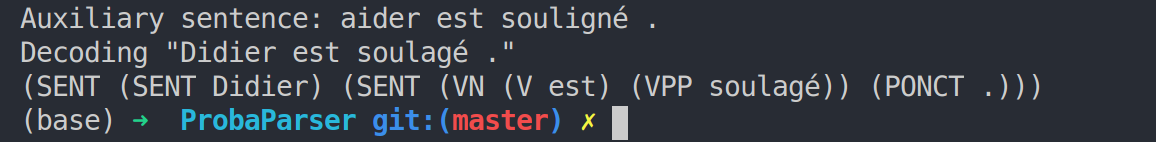
\includegraphics[width=0.7\linewidth]{didiersoulage_screenshot}
	\caption{Failure of parsing a proper noun which is out-of-vocabulary.}
	\label{fig:npParseFailure_didiersoulage}
\end{figure}


The lexical rules are transformed into a lexicon using our own \lstinline|ProbabilisticLexicon| Python class, which uses the NLTK probabilistic production data structure to represent the $(\mathrm{token}, \mathrm{PoS}, \mathrm{probability})$ triple.



\paragraph{Out-of-Vocabulary module}

There are two ways a given token $w$ can be out of the corpus vocabulary: either due to a spelling error, or actual words genuinely absent from the corpus (e.g. due to rarity).
This leads to two complementary strategies to make proposals for these words: computing \textbf{spelling} nearest neighbors in the corpus according to the Levenshtein Edit distance, and computing \textbf{semantic} nearest neighbors according to the cosine distance of some embeddings (and intersecting with the corpus vocabulary).

For the Levenshtein-nearest neighbors, we run through the corpus and compute all the distances, and get the $k$ elements with the lowest distance (without sorting).

For the embedding (semantic) nearest neighbors, we use Scikit-Learn's nearest neighbors implementation \cite{scikit-learn} (which uses search trees and is very efficient), which we fit on normalized embedding vectors using the Euclidean metric. Indeed, the Euclidean distance between normalized vectors is equivalent to the cosine distance because $\|\frac{x}{\|x\|} - \frac{y}{\|y\|}\|^2 = 2 - 2\langle \frac{x}{\|x\|}, \frac{y}{\|y\|}\rangle$.

In order to score the combined list of proposals, we use a language model trained on the corpus. We use NLTK's language modeling API to extract unigrams and bigrams from the corpus and assign appropriate weighted scores (averaging between bigram and unigram scores).

\printbibliography{}


\end{document}